\chapter{Results}
\label{chapter: Results}
% \noindent This covers an area different from the 'Testing'
% chapter, and relates to the understanding and analysis
% of the algorithm, program, or hardware behaviour.
% Where the deliverable is a product with easily
% quantified performance then the previous Chapter
% shows how functional correctness is established,
% while this Chapter shows qualitatively or
% quantitatively how well the product works. The list
% below shows typical content, not all of this will be
% applicable to all projects. \\

% \noindent An empirical relationship between
% parameters and results may be investigated,
% typically through the use of appropriate
% graphs. \\
% Where theory predicts aspects of
% performance the results can be compared 
% with expectation and differences noted and (if
% possible) explained. \\
% Semi-empirical models of behaviour may be
% developed, justified, and tested. \\

% \noindent The types of experiments/simulations that
% were carried out should be described. Why
% were certain experiments carried out but not
% others? What were the important parameters
% in the simulation and how did they affect the
% results? If there are very many graphs and
% tables associated with this chapter they may
% be put in the Appendix, but it is generally
% better to keep these close to the text they
% illustrate, as this is easier for the reader.

\section{Prediction Results}
Two main comparisons were made in order to gauge the performance of the implemented methods. The simple prediction methods were compared to previous machine learning based attempts as well as the current implementation of the Behavioural Control Theory. Both comparisons were based solely on the accuracy of prediction. Accuracy was quantitatively measured by the errors presented in Section \ref{section: errors}.

\subsection{Simple Predictions vs Machine Learning}

In an effort to form a fair comparison between the methods, the same data set, normalized in an identical way, was used. The prediction made was one day ahead and is updated every day as a moving window. The sample is from the stock \textbf{APPLE} over the period \textit{"09-07-2016"} to \textit{"09-07-2021"}, consistent with \cite{ml_paper}. This means that the training data would be \textbf{839 days} long and the testing/validation data would be \textbf{420 days} long.

\noindent Figures \ref{fig: lag_1}, \ref{fig: sma_3} \& \ref{fig: lin_3} show the graphs generated for 
a small portion (\textbf{150 days}) of the predictions and test data  in order to give a better visual representation of the difference in prediction method as it is difficult to differentiate when the entire data set is plotted. To view the plots of the entire data set, see Figure \ref{fig: full_simple} in the appendix.

\begin{figure}[h]
    \centering
    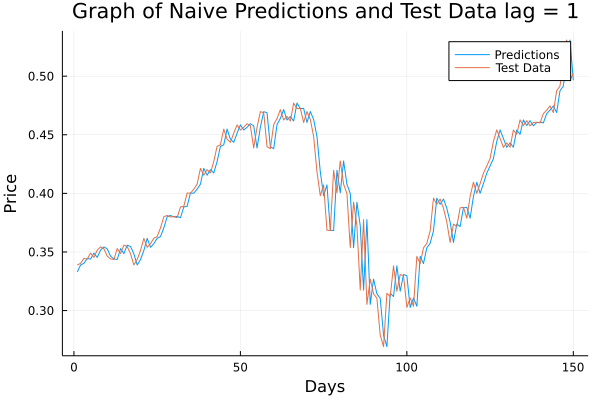
\includegraphics[width=0.8\columnwidth]{Results/lag_1.png}
    \caption{Naive Prediction and Test Data}
    \label{fig: lag_1}
\end{figure}

\noindent Figure \ref{fig: lag_1} demonstrates the Naive prediction in action with $n = 1$ - See Equation \ref{eqn: naive}.

\begin{figure}[h]
    \centering
    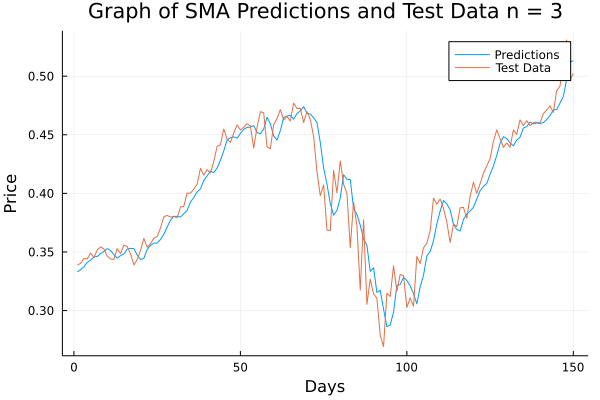
\includegraphics[width=0.8\columnwidth]{Results/sma_3.png}
    \caption{SMA Prediction and Test Data}
    \label{fig: sma_3}
\end{figure}

\noindent Figure \ref{fig: sma_3} demonstrates the SMA prediction in action with $n = 3$ - see Equation \ref{eqn: pred_sma}.

\begin{figure}[h]
    \centering
    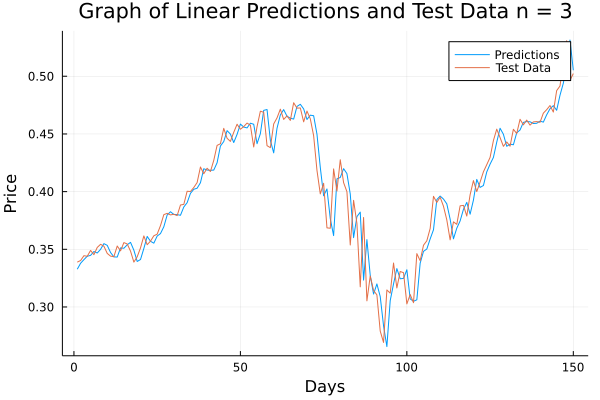
\includegraphics[width=0.8\columnwidth]{Results/lin_3.png}
    \caption{Linear Prediction and Test Data}
    \label{fig: lin_3}
\end{figure}

\noindent Figure \ref{fig: lin_3} demonstrated the Linear prediction in action with $n = 3$ - see Equation \ref{eqn: pred_lin}. 

\noindent In terms of the machine learning based attempts, the three main architectures used were \cite{ml_paper}:

\begin{itemize}
    \item Deep Neural Network (DNN)
    \item Long Short Term Memory (LSTM)
    \item Recurrent Neural Network (RNN)
\end{itemize}

\noindent Figure \ref{fig: machine} shows the plots of predictions and test data for architectures described above for the entire data set, All figures retrieved from the previous year's report \cite{ml_paper}. 

\begin{figure}[h]
  \centering
  \subfloat{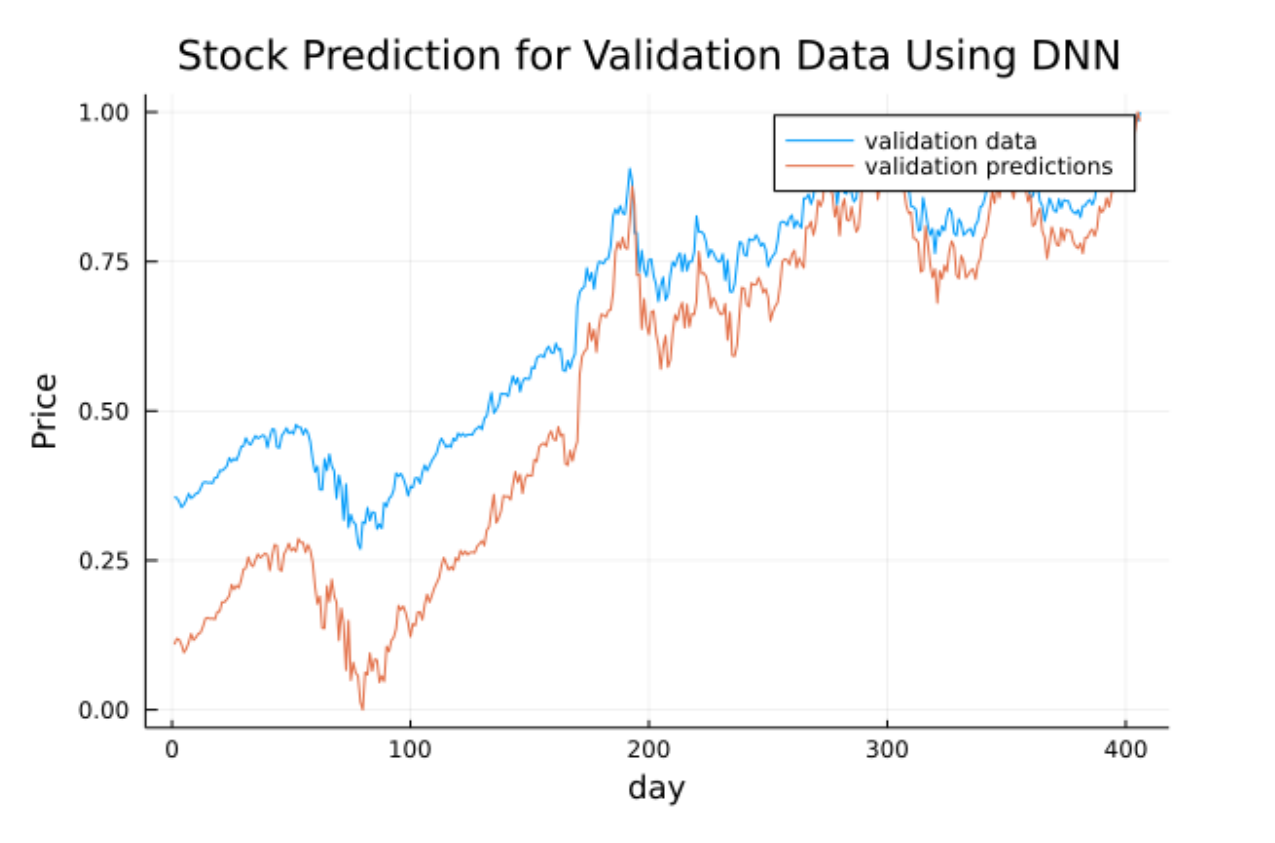
\includegraphics[width=.45\columnwidth]{Results/machine_learning_dnn.PNG}}\quad
  \subfloat{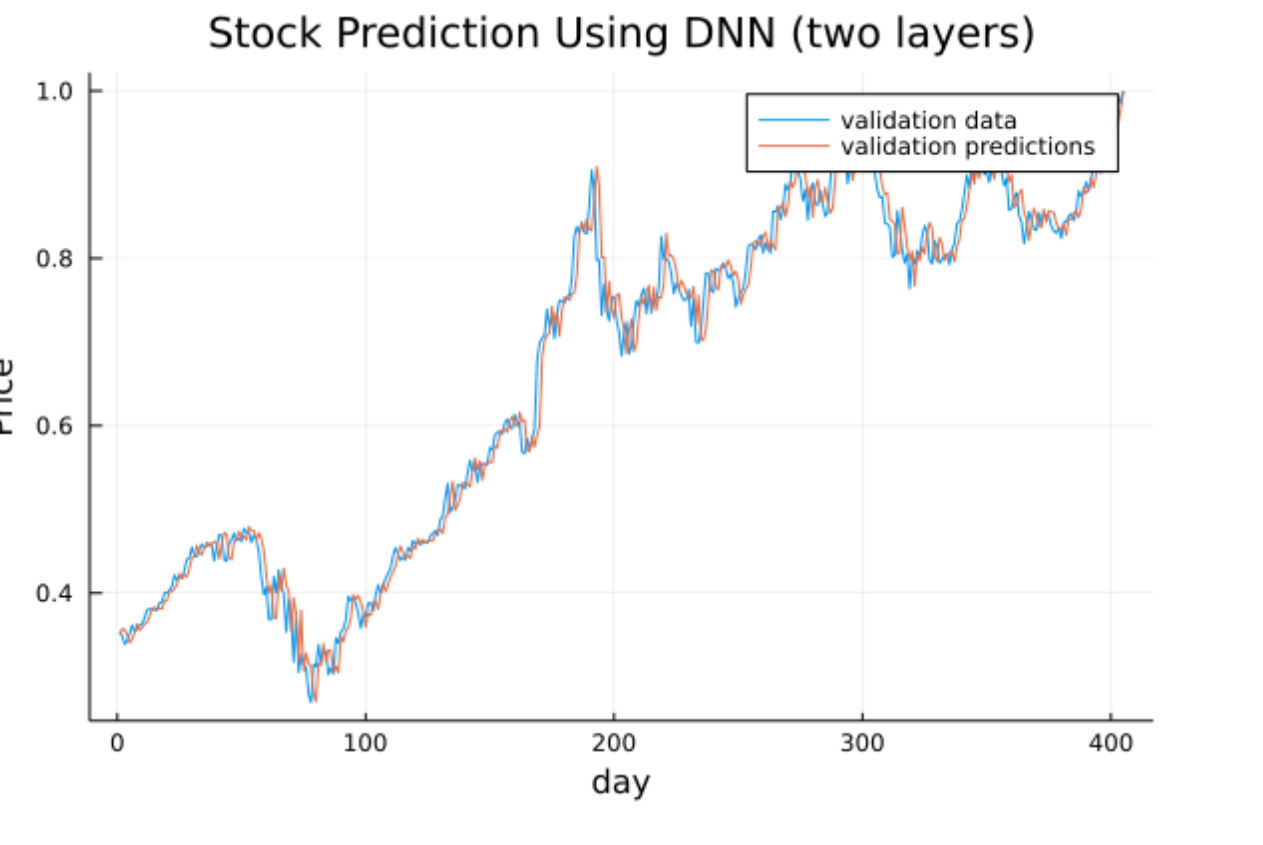
\includegraphics[width=.45\columnwidth]{Results/machine_leanring_dnn2.PNG}}\\
  \subfloat{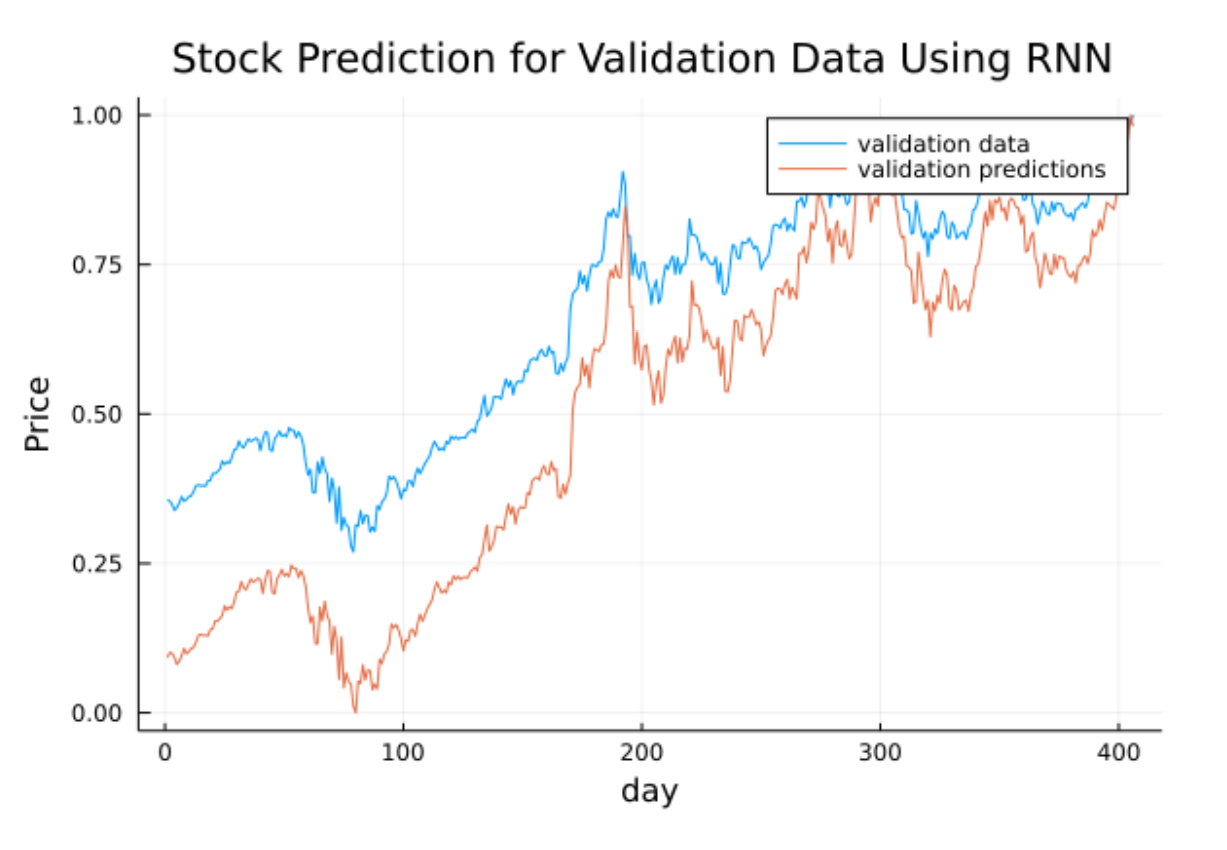
\includegraphics[width=.45\columnwidth]{Results/machine_learning_rnn.PNG}}\quad
  \subfloat{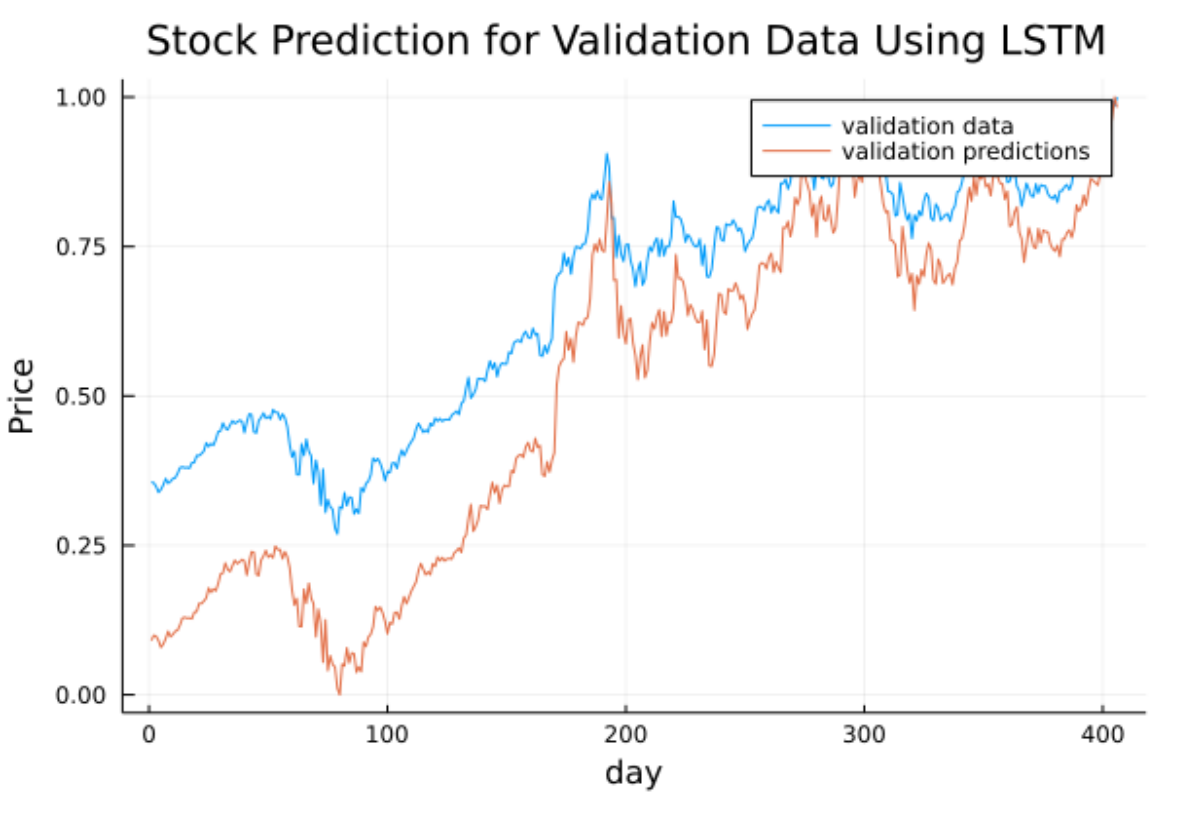
\includegraphics[width=.45\columnwidth]{Results/machine_learning_ltsm.PNG}}
  \caption{(a)DNN 1-Layer, (b)DNN 2-Layer, (c)RNN, (d)LSTM} \cite{ml_paper}
  \label{fig: machine}
\end{figure}

\noindent In terms of a numerical comparison, the mean-squared error (MSE) was calculated for each simple prediction method and compared to lowest MSE values reported for each formulation of the machine learning architectures used, this is summarized in Table \ref{tab: simp_ml_mse}. 

\noindent The complete table of all MSE values for each different formulation of ML Architecture can be viewed in Figure \ref{fig: full_machine}.

\begin{table}[h]
\begin{center}

\begin{tabular}{llll|llll}
\hline
     & \multicolumn{3}{l|}{Simple Methods}                                & \multicolumn{4}{c}{ML Architectures}                                                                       \\ \hline
     & \multicolumn{1}{l|}{Naive}  & \multicolumn{1}{l|}{SMA}    & Linear & \multicolumn{1}{l|}{DNN 1 Layer} & \multicolumn{1}{l|}{DNN 2 Layer} & \multicolumn{1}{l|}{RNN}    & LSTM   \\ \hline
    \multicolumn{1}{l|}{MSE} & \multicolumn{1}{l|}{0.0037} & \multicolumn{1}{l|}{0.0051} & 0.0037 & \multicolumn{1}{l|}{0.3093}      & \multicolumn{1}{l|}{0.3098}      & \multicolumn{1}{l|}{0.3101} & 0.3066 \\ \hline
\end{tabular}
\label{tab: simp_ml_mse}
\caption{Numerical Comparison of MSE Values between Simple and ML Architectures}
\end{center}
\end{table}

\noindent A visual comparison between Figures \ref{fig: machine} \& \ref{fig: full_simple} as well as the numerical values of MSE presented in Table \ref{tab: simp_ml_mse} suggest that previous ML based attempts did not outperform simple methods of prediction and thus, there was cause to investigate Behavioural Control Theory as a new method of prediction.

\subsection{Simple Predictions vs Behavioural Control Theory}
\label{section: simp_vs_behave}

The sample data was taken from the stock \textbf{Amazon} over the time period \textit{"2018-01-01"} to \textit{"2020-12-31"}. The reason for choosing this data set can be found in section \ref{section: data_prep}. Plotting and error evaluation were the two methods of comparison used. The predictions were generated from a range of different Hankel matrix depths ($L$) and optimisation parameter ($\gamma$) values  - see Equation \ref{eqn: opt}. 

\noindent Figure \ref{fig: simple_1_day} shows the Naive, SMA, and Linear predictions plotted with the test data for a one day ahead prediction. The parameters chosen were $n=1, n=3$ and $n=3$ respectively. 

\noindent Figure \ref{fig: behave_1} shows the behavioural prediction results for $L = 10, 20$ and variable $\gamma$. A range of different depth values for the Hankel matrix were tested, and plots can be viewed in Appendix \ref{app: first}. 

\begin{figure}[h!]
  \centering
  \subfloat{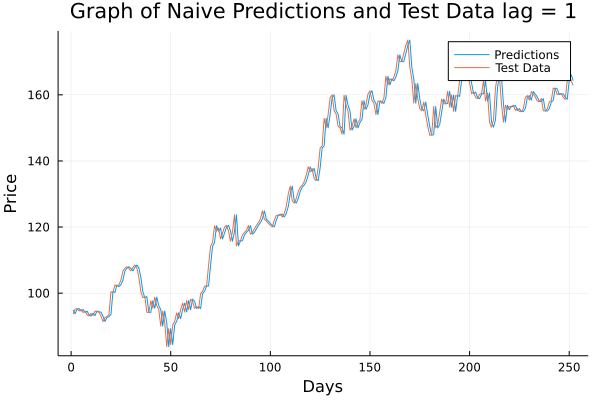
\includegraphics[width=.45\columnwidth]{Results/Simple_vs_Behavioural/lag_app_1.png}}\quad
  \subfloat{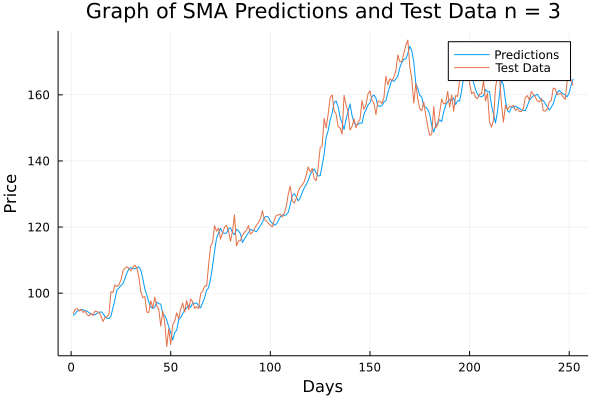
\includegraphics[width=.45\columnwidth]{Results/Simple_vs_Behavioural/sma_app_3.png}}\\
  \subfloat{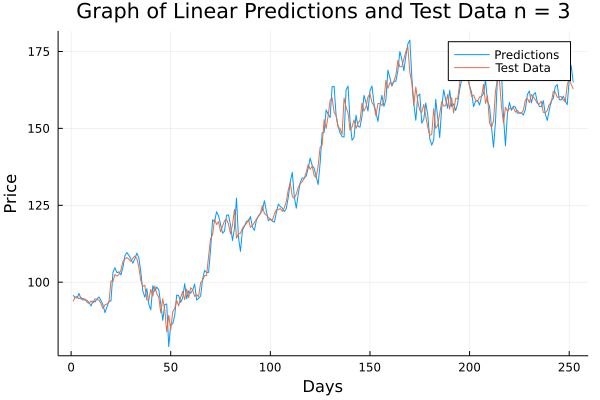
\includegraphics[width=.45\columnwidth]{Results/Simple_vs_Behavioural/lin_app_3.png}}\quad
  \caption{(a)Naive $n=1$, (b)SMA $n=3$, (c)Linear $n=3$}
  \label{fig: simple_1_day}
\end{figure}

\begin{figure}[h!]
  \centering
  \subfloat{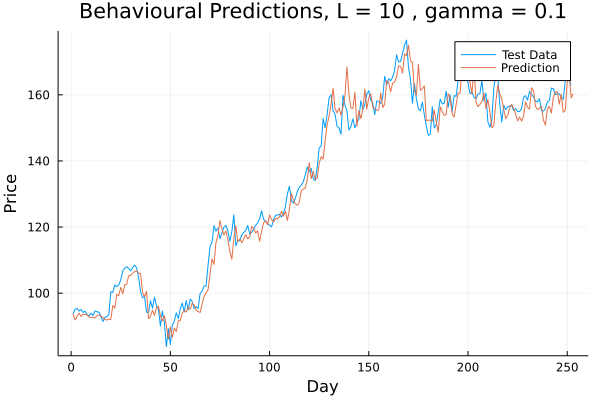
\includegraphics[width=.45\columnwidth]{Results/Simple_vs_Behavioural/depth_10_gamma_1.png}}\quad
  \subfloat{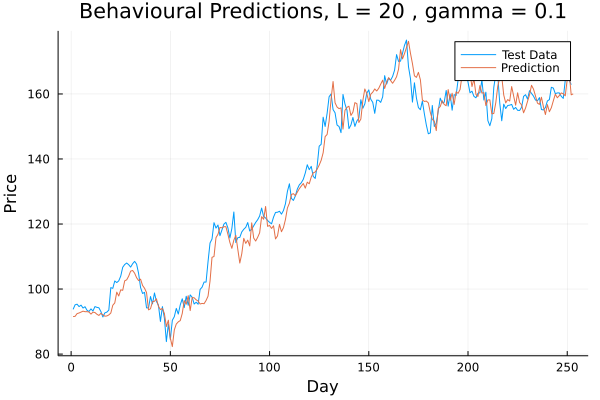
\includegraphics[width=.45\columnwidth]{Results/Simple_vs_Behavioural/depth_20_gamma_1.png}}\\
  \subfloat{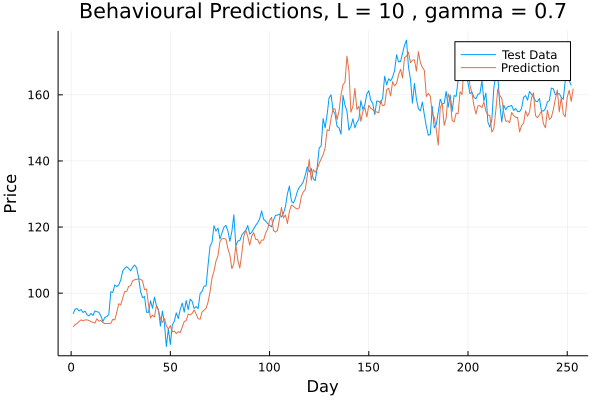
\includegraphics[width=.45\columnwidth]{Results/Simple_vs_Behavioural/depth_10_gamma_4.png}}\quad
  \subfloat{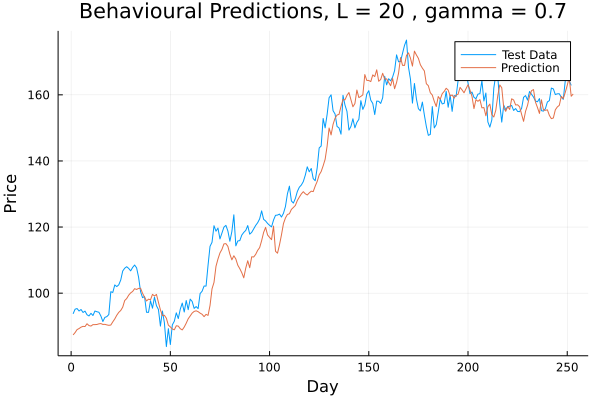
\includegraphics[width=.45\columnwidth]{Results/Simple_vs_Behavioural/depth_20_gamma_4.png}}
  \caption{(a)$L=10$ $\gamma=0.1$, (b)$L=20$ $\gamma=0.1$, (c)$L=10$ $\gamma=0.7$, (d)$L=20$ $\gamma=0.7$}
  \label{fig: behave_1}
\end{figure}

\noindent Tables \ref{tab: simple_mse_behave} \& \ref{tab: behave_mse_simple} summarize the MSE and MAE values for the Simple and Behavioural Control implementations. All MSE and MAE values were calculated on re-scaled data as it was previously standardised for processing by the Behaviour Control Theory algorithm. Although the values tested suggest that the Simple methods outperform the behavioural control implementation in terms of prediction accuracy for the chosen depth and optimisation parameter, the plots were only generated for a small portion of possible parameter combinations as producing more data points would be computationally expensive and time-consuming, thus more investigation needs to be done in order to determine the optimal values of depth, $L$ and $\gamma$ for a given stock which may be a possible project proposal in the future. Figure \ref{fig: MSE_vs_depth_gamma} illustrates the complex relationship between prediction accuracy and parameter values. 

\begin{figure}[h]
  \centering
  \subfloat{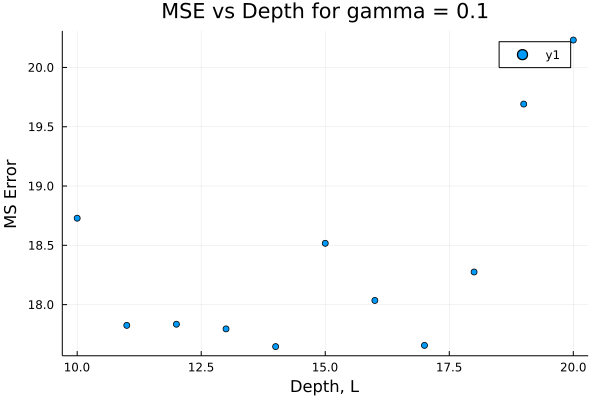
\includegraphics[width=.45\columnwidth]{Results/Simple_vs_Behavioural/MSE_vs_depth.png}}\quad
  \subfloat{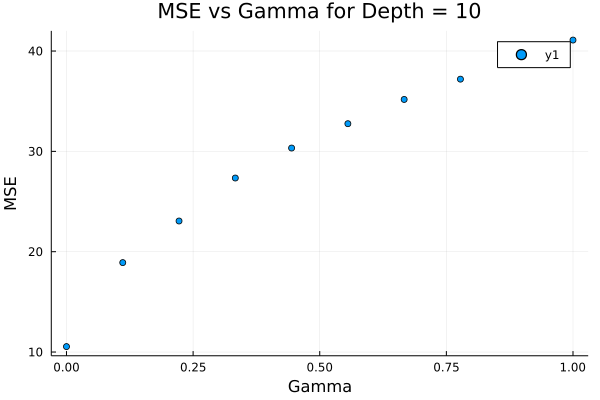
\includegraphics[width=.45\columnwidth]{Results/Simple_vs_Behavioural/MSE_vs_gamma.png}} \\
  \caption{(a)MSE vs Depth, (b)MSE vs $\gamma$} 
  \label{fig: MSE_vs_depth_gamma}
\end{figure}

\begin{table}[h!]
    \begin{center}
        \begin{tabular}{|l|l|l|}
        \hline
        Simple Method & MSE     & MAE    \\ \hline
        Naive         & 10.0801 & 2.3546 \\ \hline
        SMA           & 14.5352 & 2.8434 \\ \hline
        Linear        & 15.1152 & 2.8397 \\ \hline
        \end{tabular}
    \end{center}
    \caption{Mean Squared and Mean Absolute Error values for Simple Prediction Methods}
    \label{tab: simple_mse_behave}
\end{table}

\begin{table}[h!]
    \begin{center}
        \begin{tabular}{|l|l|l|l|}
        \hline
        Depth, L & $\gamma$ & MSE     & MAE    \\ \hline
        10       & 0.1                   & 18.7286 & 3.3840 \\ \hline
        10       & 0.7                   & 37.7373 & 4.8344 \\ \hline
        20       & 0.1                   & 20.2309 & 3.6156 \\ \hline
        20       & 0.7                   & 44.1214 & 5.4357 \\ \hline
        30       & 0.1                   & 23.8673 & 3.9093 \\ \hline
        30       & 0.7                   & 59.2911 & 6.1255 \\ \hline
        40       & 0.1                   & 33.8117 & 4.6278 \\ \hline
        40       & 0.7                   & 101.3037 & 8.2684 \\ \hline
        \end{tabular}
    \end{center}
    \caption{Mean Squared and Mean Absolute Error values for different Depth, $L$ and $\gamma$}
    \label{tab: behave_mse_simple}
\end{table}

\noindent An advantage of the behavioural control implementation is that it can compute predictions for any number of inputs. The previous predictions were generated from only raw price data, but other indicators which may be correlated with stock price movements can also be taken into account, for example volume. 

\noindent Suppose we have two vectors, $P$ and $V$ containing past values of price and volume data respectively: 

$$P = \begin{bmatrix}
p_1 & p_2 & p_3 & \hdots & p_T
\end{bmatrix} $$ 

$$V = \begin{bmatrix}  
v_1 & v_2 & v_3 & \hdots & v_T
\end{bmatrix}.$$ 

\noindent The Hankel matrix of specified depth, is constructed in the following way, 

$$ H_{L} = \begin{bmatrix}
p_1 & p_2 & \hdots & p_{T-L+1} \\
v_1 & v_2 & \hdots & v_{T-L+1} \\
p_2 & p_3 & \hdots & p_{T-L+2} \\
v_2 & v_3 & \hdots & v_{T-L+2} \\
\vdots & \vdots & & \vdots \\
p_L & p_{L+1} & \hdots & p_T \\
v_L & v_{L+1} & \hdots & v_T 
\end{bmatrix} .$$ \\

\noindent The optimisation problem is then solved as usual. Figure \ref{fig: behave_price_vol} and Table \ref{tab: mse_price_vol} illustrates a summary of the plots and error values obtained, taking into account both price and volume inputs.

\begin{figure}[h!]
  \centering
  \subfloat{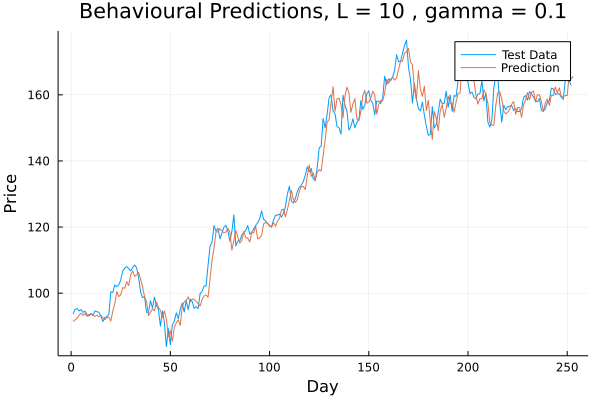
\includegraphics[width=.45\columnwidth]{Results/Simple_vs_Behavioural/Price_voldepth_10_gamma_1.png}}\quad
  \subfloat{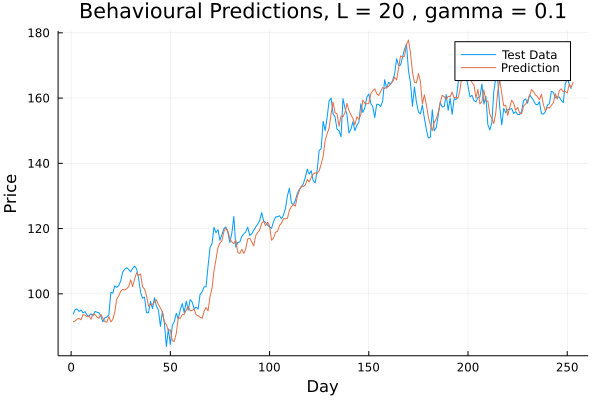
\includegraphics[width=.45\columnwidth]{Results/Simple_vs_Behavioural/Price_voldepth_20_gamma_1.png}}\\
  \subfloat{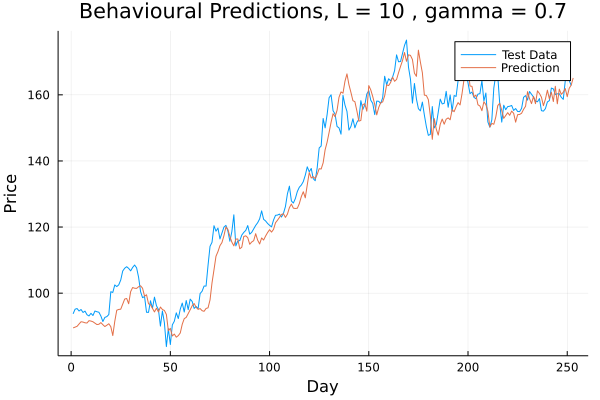
\includegraphics[width=.45\columnwidth]{Results/Simple_vs_Behavioural/Price_voldepth_10_gamma_2.png}}\quad
  \subfloat{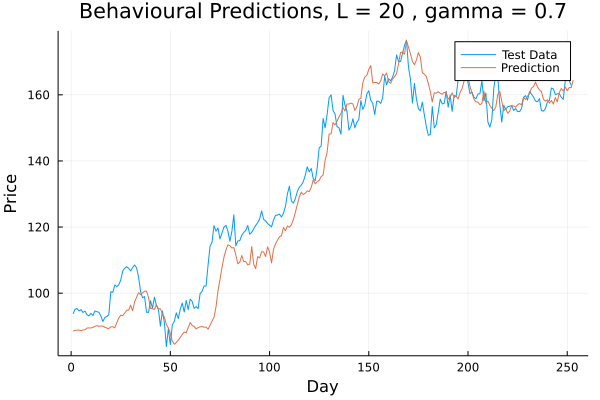
\includegraphics[width=.45\columnwidth]{Results/Simple_vs_Behavioural/Price_voldepth_20_gamma_2.png}}
  \caption{(a)$L=10$ $\gamma=0.1$, (b)$L=20$ $\gamma=0.1$, (c)$L=10$ $\gamma=0.7$, (d)$L=20$ $\gamma=0.7$}
  \label{fig: behave_price_vol}
\end{figure}

\begin{table}[h]
\begin{center}
    \begin{tabular}{|l|l|l|l|}
    \hline
    Depth, L & $\gamma$ & MSE     & MAE    \\ \hline
    10       & 0.1                   & 16.8476 & 3.1298 \\ \hline
    10       & 0.7                   & 32.1913 & 4.3784 \\ \hline
    20       & 0.1                   & 20.1726 & 3.4282 \\ \hline
    20       & 0.7                   & 60.0107 & 6.1228 \\ \hline
    \end{tabular}
\end{center}
\caption{MSE and MAE values for varying Depth $L$ and $\gamma$ values for two inputs}
\label{tab: mse_price_vol}
\end{table}

\noindent By comparing Table \ref{tab: simple_mse_behave} and \ref{tab: mse_price_vol} we can see that using multiple inputs has higher prediction accuracy for some combinations of parameters.

\clearpage

\section{Buy/Sell Strategy Results}

\noindent Although prediction accuracy is one measure of performance, investors are often interested in potential profits, therefore, a comparison needs to be made between the simple prediction methods and behavioural control implementation via the implementation of a Buy/Sell strategy. This is conducted on the same data set except, the test data is split into two portions - see Figure \ref{fig: Buy_sell},  the first half, $test\_data\_1$ is used for statistical analysis to calculate an upper and lower bound on errors. The second half, $test\_data\_2$ serves the purpose of testing the strategy - Section \ref{section: buy_sell}.

\noindent Figure \ref{fig: behave_hist} shows results of  statistical analysis for a one-day ahead prediction.

\begin{figure}[h]
    \centering
    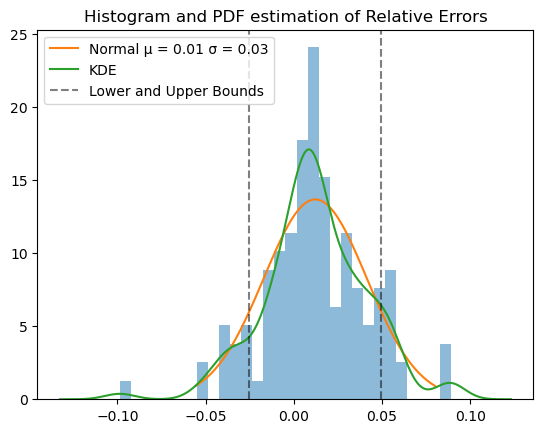
\includegraphics[width=0.8\columnwidth]{Results/Buy_sell/Behave_hist.png}
    \caption{Histogram and PDF of Relative Errors for Behavioural Control Implementation}
    \label{fig: behave_hist}
\end{figure}

\noindent The upper and lower bounds shown are the result of a user specified confidence interval of 90\%. These bounds are then used when implementing the Buy/Sell strategy. In terms of statistical analysis for the simple predictions, no upper and lower bounds were used for the SMA as they resulted little no decisions were to buy stock when testing on the data sample. If bounds were used, the total value generated was \$10,000. Additionally, implementing a buy/sell strategy for the naive prediction is not applicable as a decision cannot be made on whether to buy/sell stock if the predicted price is the same as the current. For the Behavioural Control implementation, two inputs were used to construct the Hankel matrix. A depth $L=10$ and optimisation parameter, $\gamma=0.1$ was chosen as this produced the lowest MSE as shown in Table \ref{tab: mse_price_vol} 

\noindent An initial amount of \textbf{\$10,000.00} was allocated and a standard commission of 1\% defined. Total value as well as \% Gain were calculated for the Buy/Sell strategy to be tested on the \textbf{126 days} of $test\_data2$. Additionally, a baseline was established where \textbf{\$10,000.00} was initially invested and held until the end of the period in order to gauge the performance of the market meaning, no buy/sell actions were made over the entire period. The results are summarized in Table \ref{tab: Buy_sell_1} for comparison.

\begin{table}[h]
\begin{center}
\begin{tabular}{llll|ll}
\hline
         & \multicolumn{3}{l|}{Simple Methods}                                           & \multicolumn{1}{l|}{Behavioural Control}                 & Market      \\ \hline
         & \multicolumn{1}{l|}{Naive} & \multicolumn{1}{l|}{SMA}          & Linear       & \multicolumn{1}{l|}{L = 10, $\gamma = 0.1$} &             \\ \hline
\multicolumn{1}{l|}{Total Value} & \multicolumn{1}{l|}{N/A}   & \multicolumn{1}{l|}{\$10, 512.52} & \multicolumn{1}{l|} {\$10, 115.30} & \multicolumn{1}{l|} {\$11,284.85}                                              & \$11,357.17 \\ \hline
\multicolumn{1}{l|}{\% Gain}     & \multicolumn{1}{l|}{N/A}   & \multicolumn{1}{l|}{5.13}         & 1.15         & \multicolumn{1}{l|} { 12.84}                                                   & 13.57       \\ \hline
\end{tabular}
\end{center}
\caption{Summary of Theoretical Profit for Simple vs Behavioural Methods}
\label{tab: Buy_sell_1}
\end{table}

\noindent Finally, a possible advantage of the Behavioural Control implementation is that predictions do not only have to be 1-day ahead. Predictions can be made for any number of days in the future. Thus, a Buy/Sell strategy can be implemented to make a decision "today" based on the predicted price several days into the future using the same data set up and statistical analysis technique - see Section \ref{section: buy_sell}. Most of the simple prediction methods do not have the ability to forecast several days into the future, only the Linear method produces a sensible prediction. 

\noindent Table \ref{tab: Buy_sell_2} summarizes the total value and \%gain for both Linear and Behavioural Control methods when testing the Buy/Sell strategy for predictions one week ahead of the present day, taking a standard commission of 0.1\%. 


\begin{table}[h]
    \begin{center}
        \begin{tabular}{llll|l|l}
            \hline
            \multicolumn{4}{l|}{Simple Methods}               & Behavioural Control                 & Market      \\ \hline
            \multicolumn{3}{l|}{}            & Linear         & L = 10, $\gamma$ = 0.1 &             \\ \hline
            \multicolumn{3}{l|}{Total Value} & \$9,734.46     & \$9,709.26                          & \$11,357.17 \\ \hline
            \multicolumn{3}{l|}{\% Gain}     & -2.66          & -2.93                               & 13.57       \\ \hline
            \end{tabular}
    \end{center}
    \caption{Summary of Theoretical Profits for 7 day ahead prediction}
    \label{tab: Buy_sell_2}
\end{table}

\noindent The results showcased in this chapter present some unique takeaways about the suitability of Behavioural Control Theory as a method of financial analysis to be further explored in Chapter \ref{chapter: Evaluation}. 






